%%
%%  chapter02.tex - Obstacle Detection and Planning for Autonomous Vehicles based on Computer Vision Techniques
%%
%%  Copyright 2014 Néstor Morales <nestor@isaatc.ull.es>
%%
%%  This work is licensed under a Creative Commons Attribution 4.0 International License.
%%

\graphicspath{{./images/chapter02/bmps/}{./images/chapter02/vects/}{./images/chapter02/}}

\chapter{Non-Rigid Contour Tracking}\label{ch:chapter02}

In the previous chapter, we saw a method that was able to detect obstacles as changes between the images obtained from the onboard cameras and a set of images stored in a database. We also saw that it had several drawbacks, mainly related to the localization and tracking of obstacles in world coordinates. In order to solve some of these problems, we decided to try a different solution based on a set of static monocular cameras installed all around the testing area. 
By using static cameras we can isolate the tracking problem, so other problems related to the use of onboard cameras will be left for the future. Furthermore, the obstacle detection problem becomes a foreground extraction problem, for which, as we will see next, there are many efficient solutions. 
% By doing so, we can isolate the tracking problem from the rest of problems by tracking a set of obstacles that are detected through foreground extraction methods.
Once the silhouettes of the obstacles are detected, the idea behind this method is having complete information of the trajectory followed by each point belonging to the obstacle contours. The peculiarity of our method is that the tracking is done in a non-rigid way, so we can have information about not just the moving of a certain obstacle but also about the local movement of each part of its body.
Also, as cameras are static and point to a planar surface, we assume that all obstacles lie on the ground, so their localization is quite simple. Thanks to that, we have solved some of the problems found for the method described in the previous chapter assuming an scenario in which static cameras are available. 

\begin{figure}[h!]
  \centering
  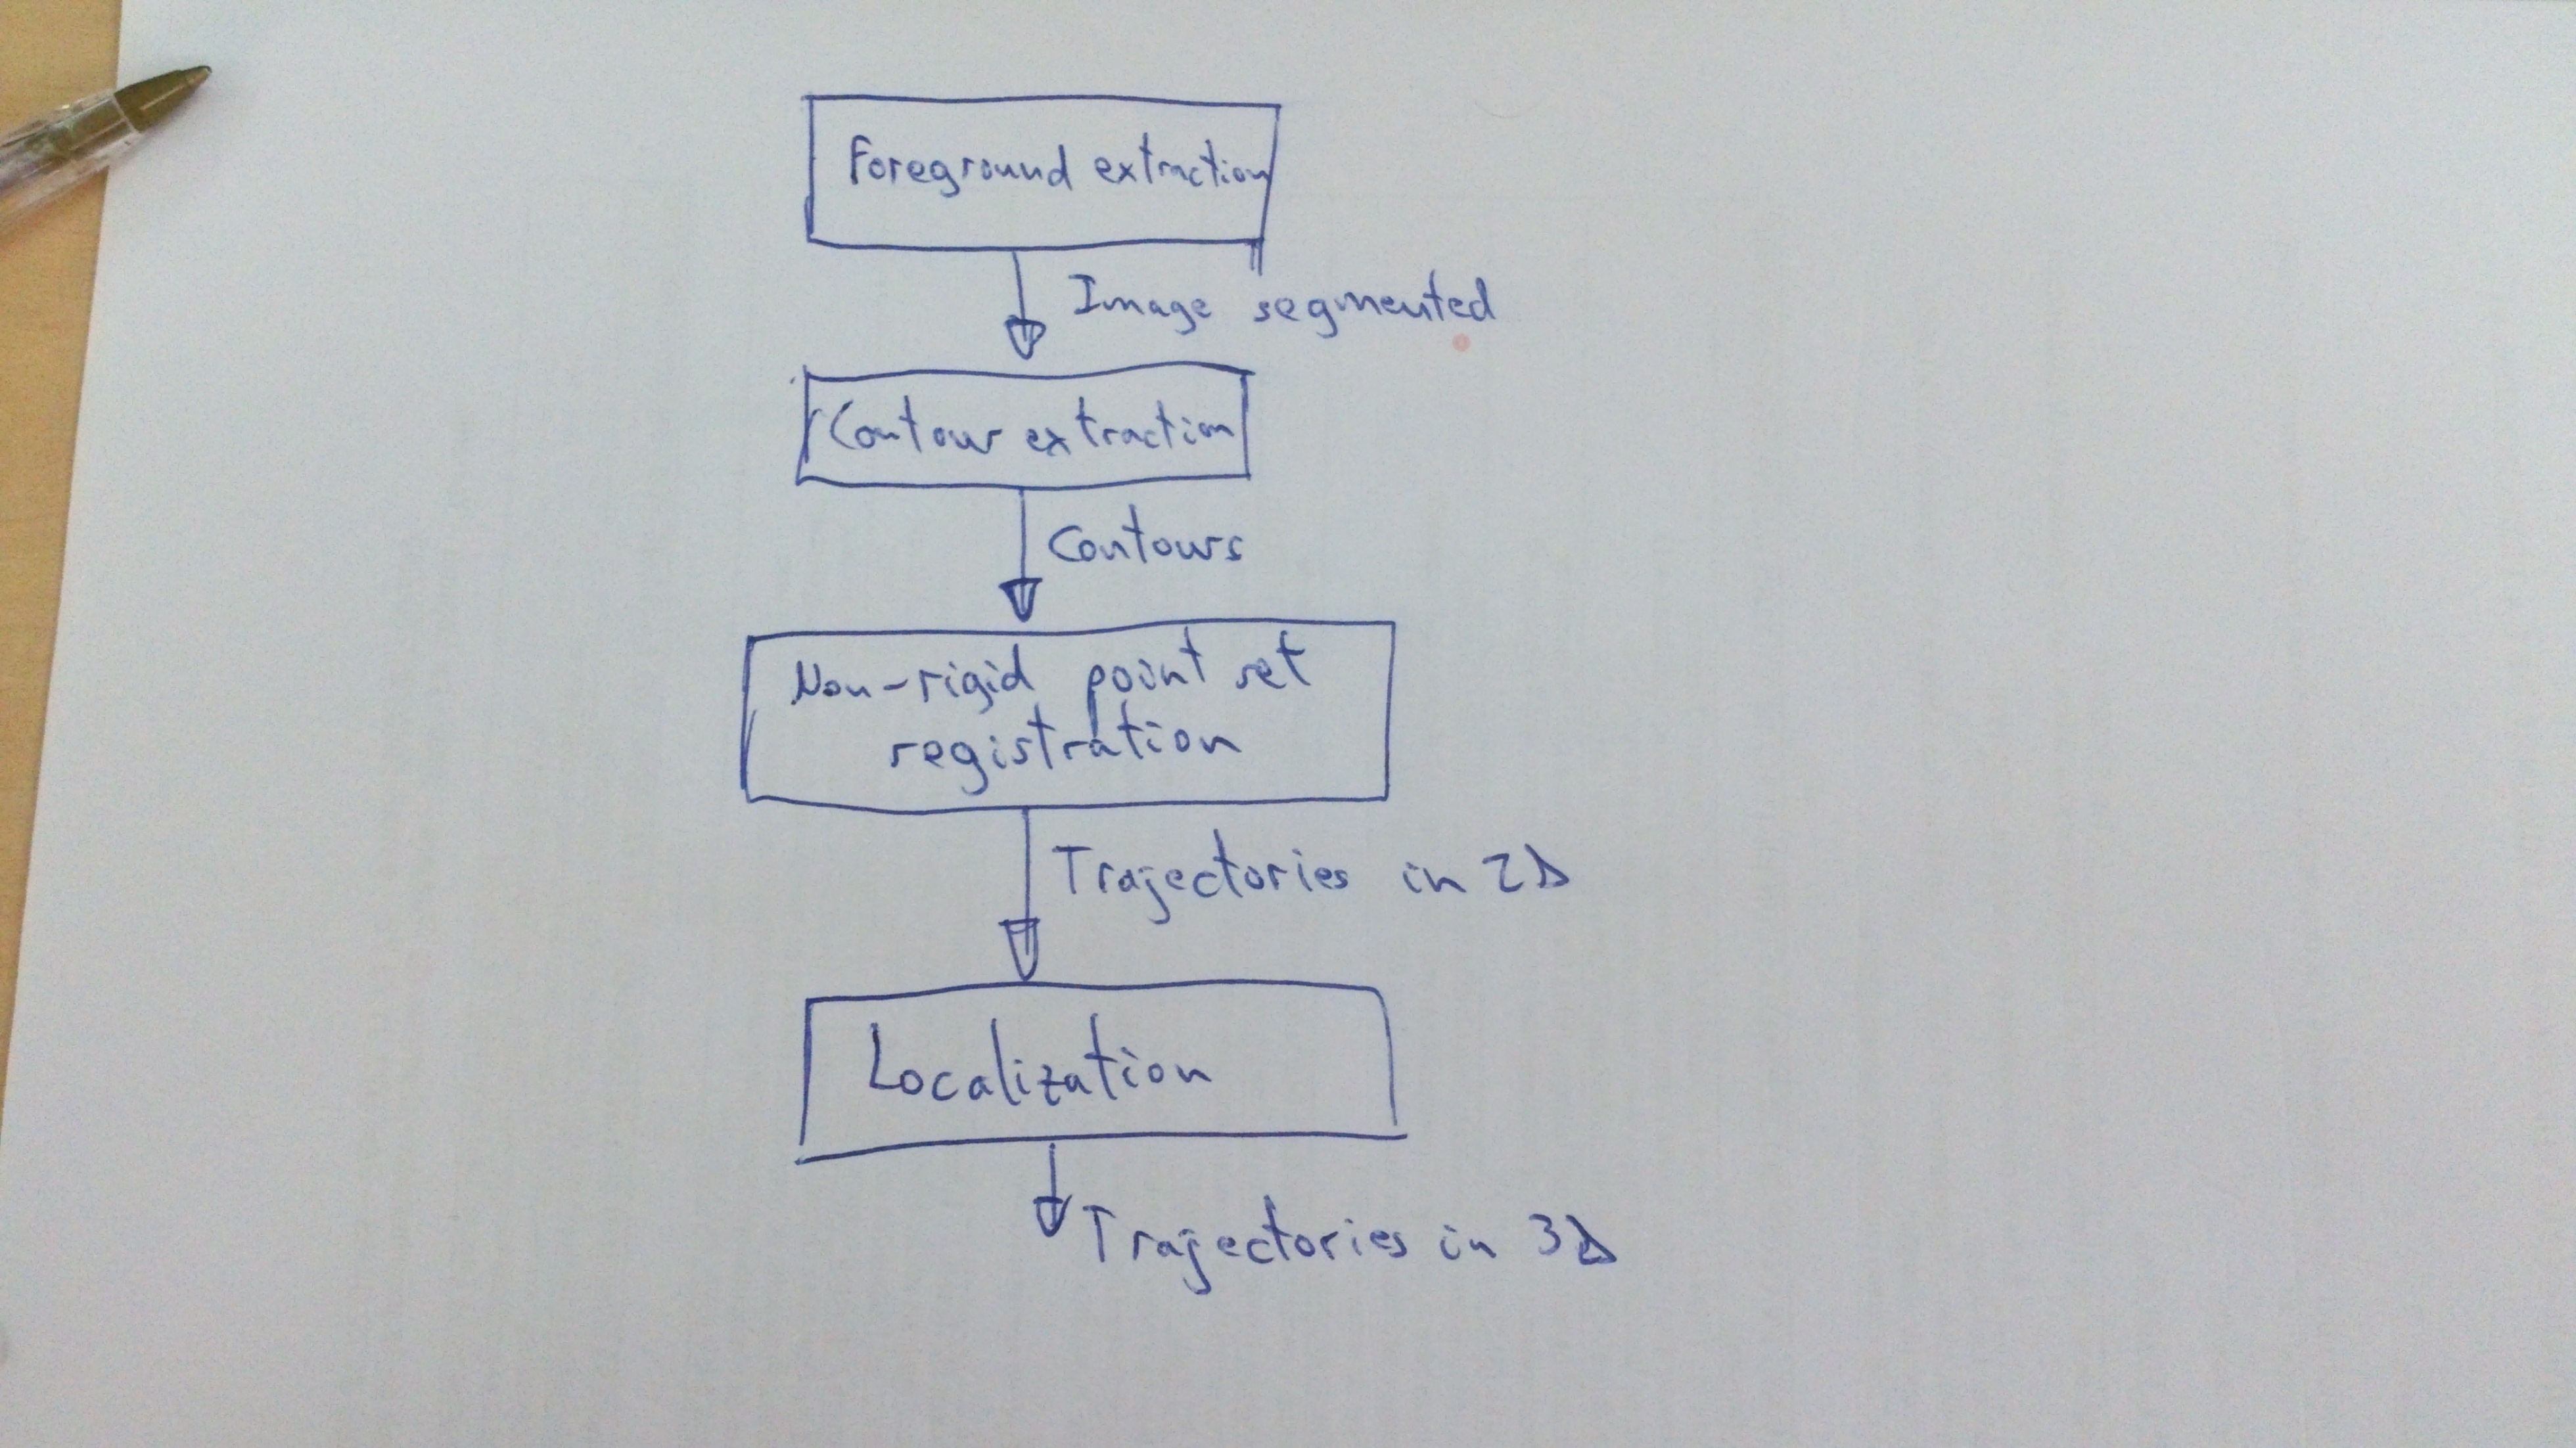
\includegraphics[width=\textwidth,height=\textwidth]{pipeline}
  \caption{Pipeline of the tracking method described in this chapter.}\label{fig:cp02_pipeline}
\end{figure}

Pipeline of the method described in this chapter is shown at figure \ref{fig:cp02_pipeline}. First, we use a method for foreground extraction in which moving objects are segmented from the background. From these objects we get the points that belong to its contour in the image. Then, a nonrigid point set registration algorithm is used to match the point pairs between each pair of frames. Concatenating these matches, it is quite easy to keep an structure in which the trajectory followed by each point in the current frame is represented. Finally, obstacles and tracks are located in world coordinates.

\section{Method}\label{ch:chapter02_01}

As seen, method pipeline can be divided into two main steps: point sets generation and contour flow detection. In the first one, we try to segment the foreground of the scene in order to extract the moving objects. Then, boundaries of the silhouettes of these objects are obtained and a non-rigid point set registration method is used to align the borders of the objects along the sequence. Finally, we obtain the trajectory followed by each part of the object contour through the time.

In the following subsections, the different stages of the algorithm are described in detail, as well as different methods we considered as candidates to perform these steps.

\subsection{Point sets generation}\label{ch:chapter02_01_01}

The objective of this step is the segmentation of those parts of the image that do not belong to the background. This stage is critical: the silhouettes must be similar enough between frames to ensure that matches between contours are correct and to help the method to converge in just a few iterations. Also, although some of the nonrigid point set registration techniques described later are able to deal with noise, it is desirable to get silhouettes as clean as possible. From these silhouettes, sets of points belonging to the contour are extracted. That is, from the current image, we obtain the point set $Y$, which will be registered with the point set obtained from the previous frame, $X$.

\subsubsection{Foreground extraction algorithms}\label{ch:chapter02_01_01_01}

For the extraction of the foreground, there are several approaches suitable for our method and able to extract the objects without a previous model of the objects that we want to extract. This is one of the objectives desired for our method. For this purpose, we have studied four different methods, described in \cite{lopez2011stochastic}, \cite{lopez2011foreground}, \cite{guo2011hierarchical} and \cite{reddy2012improved}. In this section, we do a brief introduction of these methods. In section \ref{ch:chapter02_02_01}, they are compared using a dataset for which the ground-truth is available.
The studied foreground detection methods are introduced next:

\begin{itemize}
\item \textit{BACKground Stochastic Approximation (BACKSA)}: this method is based on the work described by 
\cite{lopez2011stochastic}. This method proposes an statistical approach for background modeling and foreground 
segmentation. To do that, a mixture of probabilistic models at each pixel location is used for modeling the background and 
foreground distributions, respectively. For the background, a Gaussian distribution is used, while the foreground is 
modeled by a Uniform distribution. The initial model is afterwards fine tuned using a learning algorithm. This 
learning algorithm based on the Robbins-Monro stochastic approximation has a low computational complexity, making this method suitable for real time applications.
\item \textit{Foreground detection with Self-Organising Maps (FSOM)}: this method is described at 
\cite{lopez2011foreground}. It is an interesting Artificial Neural Network based alternative. In this 
work, background is modeled through probabilistic self-organising maps. This allows modeling background pixels with 
more flexibility. A statistical correlation measure is also used to test the similarity among nearby pixels. This 
measure provides feedback to the process, enhancing the detection performance.

First of all, a model must be defined. As mentioned above, it is based on a probabilistic self organising map, which 
accepts input pixels of any color space with a space dimension equal to 3. The likelihood of the observed data (pixel 
color value) at a given pixel position is modeled by a two components mixture probability density function.
Then, model parameters are learned again by means of the Robbins-Monro stochastic approximation algorithm. A method for avoiding 
suboptimal solutions based on the correlation measurement is also used.
\item \textit{Hierarchical ForeGround detector (HierFG)}: This is described at \cite{guo2011hierarchical}. It uses a 
hierarchical scheme supported by block-based and pixel-based codebooks. Block Truncation Coding (BTC) scheme (a 
traditional compression scheme) is extended,by dividing the image into non-overlapping blocks and representing them with 
a set of 12 intensity values. With the block-based background modeling, foreground is efficiently detected, but with a 
low precision. The pixel-based codebook strategy enhances this accuracy, at a low computational cost. Also, 
this hierarchical structure allows a good performance even if the background is not completely still.

All this solves the problem of non-stationary background and global illumination changes, while obtaining good 
results in detection and precision.

A color model is used, which allows distinguishing if a non-background pixel is indeed a shadow, highlight or 
foreground. This color model can be changed. In the tests, the model used was the same described in the original work 
\citep{carmona2008new}, as it gave good results. 
Finally, a short-term information model is used to overcome the non-stationary background problem. All these advantages make this method highly suitable for the purposes of the foreground segmentation stage, which is supported by the tests described at section \ref{ch:chapter02_02_01}. Based on these tests, a block size of $12\times12$ was used.
With this method, silhouettes are extracted. As said, the method is able to detect foreground, highlights and shadows. Just the foreground mask is needed.
\item \textit{Block-based Classifier Cascade with Probabilistic Decision Integration (BCCPDI)}: The last method 
considered is based on the work of \cite{reddy2012improved}. In the HierFG approach, we introduced a hierarchical 
algorithm in which data is analyzed from two different viewpoints (region and pixel levels). This methodology 
tackles frames as composed by a number of overlapping blocks.

The method is composed by four main stages:
\begin{itemize}
 \item In the first stage, a given image is divided into overlapping blocks. For each block, a low-dimensional texture descriptor is generated, which is passed to a cascade classifier.
 \item Each block is classified as background or foreground using the cascade classifier, comprising three 
classifiers, each one managing a different problem: the first one is able to handle dynamic backgrounds, but 
fails in presence of illumination variations; the second one detects whether the anomalies found in the previous 
descriptor are generated by illumination variations; and the third descriptor is able to exploit temporal correlations. 
By doing that, it is able to partially handle changes in environmental conditions while reducing spurious false 
positives.
 \item If a portion of each image is consistently classified as foreground for a reasonable period of time, the 
stage "model reinitialization" is triggered. This happens when a sudden and significant scene change is too sudden or 
too severe for the adaptation and classification strategies being followed. This can make the current background model 
inaccurate, which leads to the detection of a very large portion of the image as foreground.
 \item In the final stage, a probabilistic approach for the generation of a foreground mask is used. This approach 
exploits the block overlaps in order to integrate the decisions at block-level, obtaining a pixel-level final 
foreground segmentation. In this stage, each pixel is classified as foreground only if a significant proportion of the 
blocks that contain that pixel are classified as foreground. This strategy minimizes the number of errors in the 
output. This is in contrast to conventional methods, such as those based on Gaussian Mixture Models, Kernel Density 
Estimation and Codebook Models, which do not include this correction stage.
\end{itemize}

This method also presents some advantages that make it very suitable for our application:
\begin{itemize}
 \item First of all, as happened with the previous method, it is able to deal with illumination changes and dynamic backgrounds. The use of a cascade classifier makes it very robust, as in the second classifier it is able to distinguish if the detected change was motivated by a real movement of a foreground object or it was caused by a change in the illumination. The remaining false positives are removed by the third classifier.
 \item In second place, soft contours are found. As shown in section \ref{ch:chapter02_02_01}, these contours are pretty much softer than those obtained by other methods. As the presented application is very sensitive to a bad detection of these contours, this is a key feature.
 \item It is able to work even with dynamic backgrounds. As the application will be working outdoors, this is also an important feature. This will allow the final application to work in areas where there are trees or other non static objects that could make the method fail.
 \item It works even in presence of noise. This is a good feature, as it will make the present method stronger.
\end{itemize}
 
\end{itemize}

In the final version of the application, and after performing the tests described at section \ref{ch:chapter02_02_01}, the algorithm chosen for the foreground detection was BCCPDI. It was not a clear decision, and in fact, some of the other methods, like FSOM, could be used instead.

\subsubsection{Point set extraction}\label{ch:chapter02_01_01_02}

The next step in this stage is obtaining the points that compose the contour of the objects represented in the mask. This is done by using the method described at \cite{suzuki1985topological}. With this method, a new point cloud is obtained, so we now have two point sets. The first one, obtained in the previous frame, is $X$; the second one is the set $Y$. In the next step, an algorithm will be used to perform a non-rigid registration between $X$ and $Y$, which will allow matching each point $x \in X$ to its corresponding point $y \in Y$. After this registration, a matching process will be performed. Results of this matching, through the frames, will return the trajectory followed by each point in the contour of the tracked objects.

\subsection{Contour flow detection}\label{ch:chapter02_01_02}

At this point, at each frame, a pair of point sets is available. Both sets, obtained in the previous step, represent a pair of shapes (or a pair of shape sets, in case there are more than one object in the scene). Also, assuming that the frame rate is high, these shapes will be similar enough to be able to find correspondences between the different points that belong to the contours by using just their spatial configuration. 

Assuming that there will not be a big change between frames, it is permissible to think that this condition will be fulfilled, and that it is possible to match the contour points by using a non-rigid point set registration based method, without the need of visual information.

\subsubsection{Non-rigid point set algorithms}\label{ch:chapter02_01_02_01}

In the literature, some non-rigid point set registration methods are described. In \cite{myronenko2010point}, a complete review of both rigid and non-rigid existing methods is enumerated. For the development of the application described here, some of these have been tested, including some others:

\begin{itemize}
 \item \textit{Iterated Closest Point (ICP) \citep{besl1992method, feldmar1996rigid}}: The method tested 
is not the original ICP algorithm, but an improved version of it. This version is thought to allow non-rigid surface 
registration. Method is divided in three different steps: in the first step, the best rigid displacement is searched 
in order to superpose both point sets; then, the best affine transformation is obtained. In this step, a global 
criterion minimized by extended Kalman filtering is used in order to ensure the convergence of the algorithm.; finally, 
each point is attached to a local affine transformation with the purpose of deforming the point set at a local level. 
 \item \textit{Thin-Plate Splines Robust Point Matching (TPS-RPM) \citep{chui2000new}}: This approach uses a Thin-Plate Spline (TPS) kernel that contains the information about the point-set's internal structural relationships and generates a non-rigid warp.
 It alternates the update of the mapping and correspondence parameters, in the way that both solutions mutually improve one another during the process until convergence is reached. In order to ensure that the method converges towards a solution, instead of getting worse, two techniques are used: the first one is soft assign, which consists on employing a variable continuous in the space inside the interval [0, 1], instead of a binary one; the other technique is called deterministic annealing, closely related to simulated annealing and described in \cite{geiger1991parallel}.
 \item \textit{\acf{CPD} \citep{myronenko2010point}}: It is a multidimensional probabilistic robust registration method that can be used for the matching of both rigid and non-rigid point sets. This algorithm defines the alignment of two point sets as a probability density estimation problem, where a point set represents the centroids of the \ac{GMM} and the other represents data points. Coherent Point Drift considers the alignment of two point sets as a probability density estimation problem, where one point set represents the model points and the other represents the data points. At the end of the process, the two point sets are aligned and the correspondence is obtained using the maximum of the \ac{GMM} posterior probability for each point. The underlying idea of the method is to force \ac{GMM} centroids to move coherently as a group to preserve the topological structure of the point sets.
 This algorithm has some advantages that make it suitable for the proposed application:
 \begin{itemize}
  \item It is able to register non-rigid large data sets. The images used in this application are not too big and just 
points in the contours are being used in order to not to increase too much the number of points. On the other hand, its 
performance is much more constant than that obtained by the other algorithms, as shown in figure 
\ref{fig:cp02_chartsRegistration}.
  \item The estimation of the \ac{GMM} width reduces the number of free parameters while reducing the number of iterations and the processing time. As situations can change, it is not desirable to use a parameter dependent algorithm. This also makes it easier to tune the whole application.
  \item It is able to simultaneously find both the transformation and the correspondences between two point sets without a previous assumption of the non-rigid transformation model except that of motion coherence. This makes unnecessary the use of a model of the objects that are expected to appear in the surveyed area.
  \item Compared to the other methods, it shows a more robust and accurate performance with respect to noise, outliers, 
and missing points. In section \ref{ch:chapter02_02_02}, it showed to have the best compromise between error, 
number of mismatches and computing time stability.
 \end{itemize}
 However, \ac{CPD} assumes no specific point correspondences other than those derived from the euclidean distances between 
points. Therefore, there are some situations in which its performance can be reduced, because the likelihood function may 
not have a well-defined maximum. Also, sometimes the use of a \ac{GMM} may be a bad choice when  
data is imperfect (i.e., the presence of outliers or missing data), leading to a fake global maximum (a local maximum) in the likelihood function. Because of that, the 
algorithm can be weak in these circumstances. For example, we could find outliers in case of a bad foreground segmentation. In this case, two masks related to the same object in consecutive frames are too different so it is difficult for the algorithm to match both contours. However, in practice, as the time between frames is small, the segmentation methods give similar masks in consecutive frames. Moreover, the small mismatches we could find are corrected in the next frame, so experimentally it does not seem to be a big deal. About missing points, this effect is more common. For example, think on an arm that disappears behind the body of a person. In this case, we will not be able to match the points belonging to this arm. Anyway, this situation will be normalized in the next frames.

 \item \textit{Robust Point Matching for Non-Rigid Shapes (RPM-NRS) \citep{zheng2006robust}}: In this solution, each 
point is considered as a node in a graph. Two nodes are connected by an edge only if they are neighbors. Based on this, 
the matching problem becomes a maximization problem. This is a hard discrete combinatorial problem, and the way used to 
solve it is through relaxation labeling.
 \item \textit{Dynamic Programming based Point Set Matching (DPPSM) \citep{lian2012rotation}}: In this approach, the 
Shape Context (SC) descriptor is used. This descriptor is very discriminative and quite robust to various types of 
disturbances, which proves to be a useful feature for this kind of methods. A graph is also 
constructed from a point set. Edges in this graph are used to determine the orientations of SCs. Similar to lengths or 
directions, oriented SCs constructed this way can be regarded as the attributes of edges. By doing that, rotation 
invariance can be achieved by matching the edges between the two point sets. As happened with the RPM-NRS, the point set 
matching problem becomes a graph matching problem. This simplifies the use of dynamic programming for optimization.
 The key is on how the graphs are constructed for both datasets. For the data point set, a complete graph is used, in 
the way that any two points are adjacent in the graph. In the case of the model point set, two different approaches are 
explored:
 \begin{itemize}
  \item \textit{Minimum Spanning Tree induced triangulation (MST)}: In this approach, there are two types of edges: the frame edges formed by choosing one point as the reference and connecting it to the rest of points; and the boundary edges generated in the MST constructed by the model points except for the reference point.
  The graph generated is a 2-tree \citep{west2001introduction}, which allows using a dynamic programming approach.
  \item \textit{Star graph (STAR)}: As MST scheme has a relatively high time complexity, authors of the method proposed an alternative scheme, which involves only the frame edges. Edges in a star graph form a tree, which still allows using dynamic programming to find the best embedding of the graph in the data point set, but with a much lower time complexity.
 The main advantage of this algorithm is its robustness to various types of disturbances, in special clutters. This is due to the strong discriminative nature of SC, combined with the special structure described for the model graphs and the global optimality obtained through dynamic programming.
 \end{itemize}
\end{itemize}

The named methods have been tested, obtaining the results shown at section \ref{ch:chapter02_02_02}. As it will be explained better in that section, best results were obtained for the Coherent Point Drift algorithm, as it was the only one which obtained good results in all parameters tested.

\subsubsection{Points matching}\label{ch:chapter02_01_02_02}

Now that we know which is the best algorithm for the problem we are tackling, the process is the following: we use 
the \acf{CPD} method to align both $X$ and $Y$ point sets. After that, we have a set 
of pairs $\Phi = \{ \phi(x,y) ~|~ x \in X, ~y \in Y \}$, in which the $L_2$ distance of each pair of points in 
$\Phi$ can not be bigger than a given threshold $\tau$. In our tests, $\tau = 1\,px$. After that, and to ensure that all correspondences are right, 
they are filtered in order to avoid that a point belonging to an object is matched with a point from other different 
object. 
The way in which this is done is the following:
\begin{itemize}
 \item First, both $X$ and $Y$ are clustered into different objects using the method in chapter 6.2 of 
\cite{rusu2009semantic}. Then we obtain two sets of point clusters: $\mathcal{C_X} = \{ X_i ~|~ i=1 \dots M \}$ 
and $\mathcal{C_Y} = \{ Y_j ~|~ i=j \dots N \}$.
 \item For each cluster $X_i$ we define a squared region $Rx_i$ delimited by the points $(x_{min}, y_{min})$ and $(x_{max}, y_{max})$, where $x_{min}$ and $y_{min}$ are the minimal $x$ and $y$ values in the set $X_i$, and $x_{max}$ and $y_{max}$ the respective maximal values. Same process is performed for each cluster $Y_j$, obtaining the region $Ry_j$.
 \item As they do in \cite{siebel2003design}, we compare each region $Rx_i$ with each region $Ry_j$, obtaining the following values: absolute positional difference in $x$ and $y$ direction ($\varDelta x$ and $\varDelta y$, respectively), absolute difference in width ($\varDelta w$), and absolute difference in height ($\varDelta h$). From these values we obtain the following matching score:
 \begin{equation}\label{eq:matching_regions}
  \delta (Rx_i, Ry_j) = \alpha_1 \varDelta x + \alpha_2 \varDelta y + \alpha_3 \varDelta w + \alpha_4 \varDelta h.
 \end{equation}
 As done in \cite{siebel2003design}, the values used for the parameters were $\alpha_1 = \alpha_1 = \alpha_3 = 1$ and $\alpha_4 = 1.5$. The weight used for the height of the tracked objects is slightly bigger because it is usually more invariant to changes in orientation.
 \item Using the score of equation \ref{eq:matching_regions}, we look for each region $Ry_j$ its nearest region $Rx_i$. 
If the score is below a threshold $\delta_{max}$, $Y_j$ will be labeled with the label $\mathcal{L}(i) = j$.
 \item Once all regions are labeled, we reject the pairs $\phi(x,y)$ in which the label of the cluster containing 
$x$ is not the same of the cluster containing $y$. In figure \ref{fig:cp02_clusterization_output}, it is possible to see a 
pair of objects crossing each other in a sequence. Each color represents a different cluster. In that sequence, two 
clusters are joined and, once the people in the image are separated again, the cluster is split into two 
different clusters. In our tests, $\delta_{max} = 100$.
\end{itemize}

\begin{figure*}[t]
        \centering
        \begin{subfigure}[b]{0.32\textwidth}
                \centering
                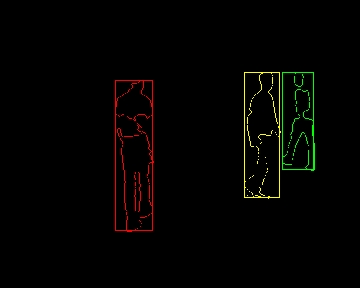
\includegraphics[width=\textwidth]{fig1.jpg}
                \caption{~}
                \label{fig:cp02_cluster1}
        \end{subfigure}%        
        ~ %add desired spacing between images, e. g. ~, \quad, \qquad etc.
          %(or a blank line to force the subfigure onto a new line)
        \begin{subfigure}[b]{0.32\textwidth}
                \centering
                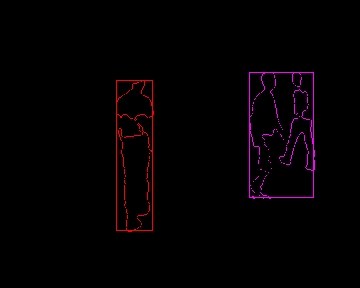
\includegraphics[width=\textwidth]{fig2.jpg}
		\caption{~}
                \label{fig:cp02_cluster2}
        \end{subfigure}%
        ~ %add desired spacing between images, e. g. ~, \quad, \qquad etc.
          %(or a blank line to force the subfigure onto a new line)
        \begin{subfigure}[b]{0.32\textwidth}
                \centering
                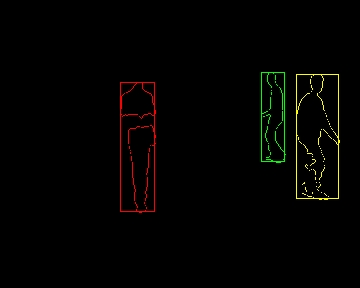
\includegraphics[width=\textwidth]{fig3.jpg}
                \caption{~}
                \label{fig:cp02_cluster3}
        \end{subfigure}%
        \caption{Clustering of objects before, during and after two of them cross each other in a sequence.}\label{fig:cp02_clusterization_output}
\end{figure*}

Pairs must be added to a structure that represents the current set of trajectories. Such structure is depicted in figure \ref{fig:cp02_trajectories_structure}. For each pair $\phi(x,y)$, we look for a point $p_{xn}$ in the list of points that are the head of the trajectories already stored in the structure, such that $p_{xn} = y$. If we found this point in the structure, we add it to the head of the associated trajectory, which is indexed through the new point $(a)$. Else, the point is added as a new trajectory $(b)$. Once all pairs have been processed, those which have not been updated are removed from the structure (represented in red in figure \ref{fig:cp02_trajectories_structure}).

\begin{figure*}[h]
  \centering
%   \includegraphics[width=0.4\textwidth, trim=180 10 100 20,clip]{finalPath.jpg}
  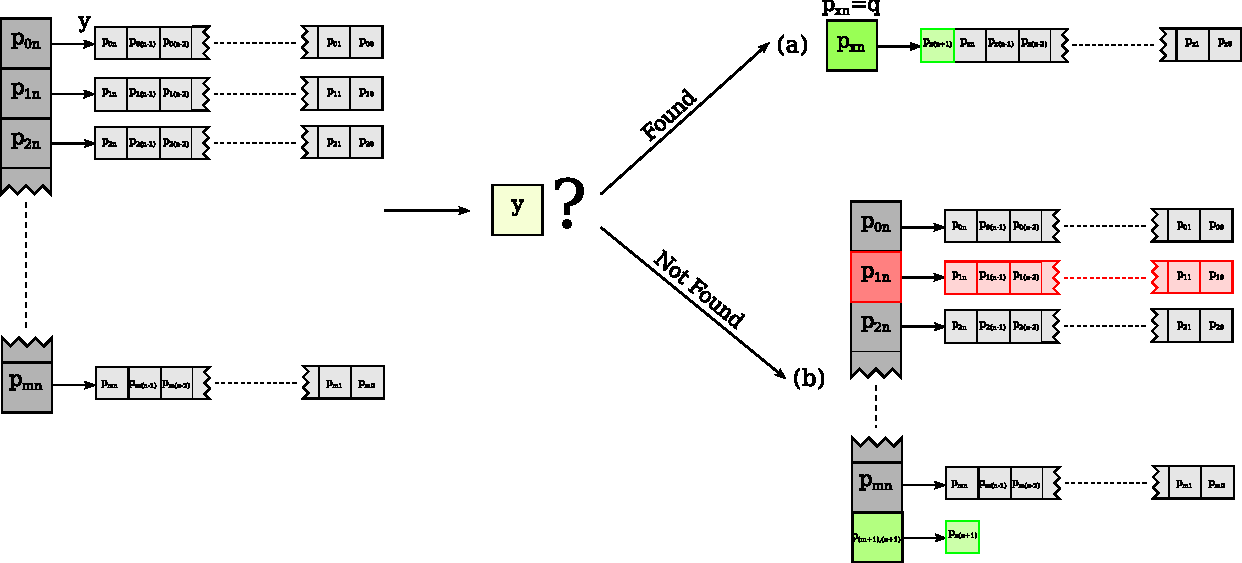
\includegraphics[width=0.7\textwidth, trim=0 0 0 0,clip]{fig4.pdf}
  \caption{Trajectories structure.}
  \label{fig:cp02_trajectories_structure}
\end{figure*}

At this point, we have all the trajectories generated and stored in a structure. This information can be used as 
input by other algorithms, i.e. in human behavior recognition, video surveillance tasks or human-computer 
interaction applications. In figure \ref{fig:cp02_videoCaptures} we show a set of frames extracted from the video available at \url{http://youtu.be/QqE_cBTM1jo}, in which it is possible to see a representation of the output obtained by our 
algorithm, as well as an explanation of the pipeline followed. For the sake of clarity, each trajectory is represented by a random different color, and not all of them 
are depicted. Images are part of the dataset used in \cite{berclaz2011multiple}, available on the 
web\footnote{\url{http://cvlab.epfl.ch/data/pom}}.

\begin{figure*}[t]
        \centering
        \begin{subfigure}[b]{0.24\textwidth}
                \centering
                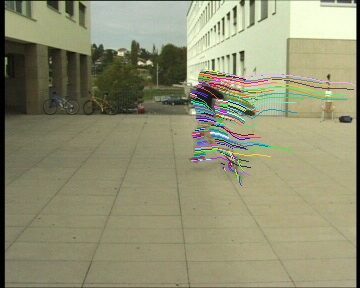
\includegraphics[width=\textwidth, trim=6 0 5 1, clip]{fig5.jpg}
                \caption{~}
                \label{fig:cp02_videoCapture1}
        \end{subfigure}%        
        ~ %add desired spacing between images, e. g. ~, \quad, \qquad etc.
          %(or a blank line to force the subfigure onto a new line)
        \begin{subfigure}[b]{0.24\textwidth}
                \centering
                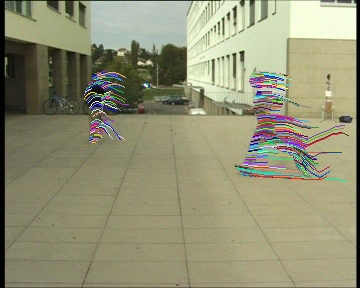
\includegraphics[width=\textwidth, trim=6 0 5 1, clip]{fig6.jpg}
		\caption{~}
                \label{fig:cp02_videoCapture2}
        \end{subfigure}%
        ~ %add desired spacing between images, e. g. ~, \quad, \qquad etc.
          %(or a blank line to force the subfigure onto a new line)
        \begin{subfigure}[b]{0.24\textwidth}
                \centering
                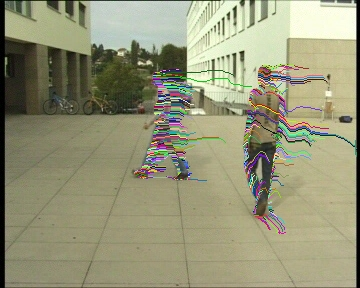
\includegraphics[width=\textwidth, trim=6 0 5 1, clip]{fig7.jpg}
                \caption{~}
                \label{fig:cp02_videoCapture3}
        \end{subfigure}%
        ~
        \begin{subfigure}[b]{0.24\textwidth}
                \centering
                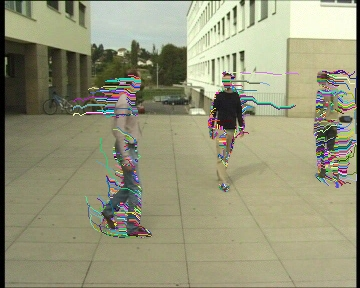
\includegraphics[width=\textwidth, trim=6 0 5 1, clip]{fig8.jpg}
                \caption{~}
                \label{fig:cp02_videoCapture4}
        \end{subfigure}%
        \caption{Captures from the attached video corresponding to the frames 1695, 1715, 3669 and 3789 of the dataset used by \cite{berclaz2011multiple}.}\label{fig:cp02_videoCaptures}
\end{figure*}

\subsection{Localization}\label{ch:chapter02_01_03}

As we are just using a single camera for the detection and tracking of the obstacles, it is not possible to know the exact location in which the obstacle is in the real world. Fortunately, used cameras are static, and it is possible to take advantage of this fact. As the area covered by each camera is known and it is assumed to be planar, a set of four virtual points can be defined over the road, for which the coordinates in the map are well known.
Having this, these points can be selected on the image. By doing a perspective projection, the objects in the image can be localized on the map. This is possible because we assume that every object is lying on the ground, touching it.

\section{Summary}\label{ch:chapter02_03}

In this chapter we have presented a method for the estimation of the trajectory followed by each part of non-rigid bodies in sequences of static images. The key features of the proposed method are:
\begin{itemize}
 \item It is able to work both indoors and outdoors
 \item It does not need any previous model of the tracked object
 \item It can track each part of the body, separately, without any previous assumptions.
\end{itemize}

With this approach, we have demonstrated that it is possible to perform the tracking of the contour with the use of just geometrical information. In our tests (see section \ref{ch:chapter02_02}), we will show that our method works even better than optical flow in certain situations. 

As future work, we plan to study the inclusion of visual information to improve the results given by the current method.

We have studied the performance of several state-of-the-art foreground extraction algorithms, shedding light on the 
benefits and drawbacks of each of them. Among all, BCCPDI is the one which fulfills the most of our needs, as we will see in section \ref{ch:chapter02_02}. 

We also have performed some tests in order to select the best of the existing state-of-the-art nonrigid point set registration methods, demonstrating that \ac{CPD} is the most stable of all them. Final tests demonstrate the good behavior of the algorithm, showing that it is possible to obtain a local tracking of nonrigid objects by just using static cameras. All these tests are described, and their results shown, at section \ref{ch:chapter02_02} of chapter \ref{ch:chapter08}.

However, the application has some unsolved challenges that must be tackled in future, mainly related to the 
limitation of using just the contours of $2D$ masks. The first of them is that if a  $2D$ mask is used, we lost any 
depth information, so it is impossible to find the contours of a first-plane object if in the image there is more than 
one object touching each other. 

Another limitation we noticed is that it is impossible to track the movement of a hand, for example, if it 
passes in front or behind of the body of a person. 

In the following chapters, we will see some approaches that make use of 3D information for the detection and tracking of the obstacles, but in a different way than that presented in this chapter. But, before that, we will see an study of the existing techniques available for stereo reconstruction oriented to \ac{ADAS} applications.

% All these problems can be overcome with the use of $3D$ point clouds as input for the nonrigid point set registration 
% algorithms obtained with an stereo pair. This can be achieved easily, as most of the presented methods are able to work 
% with $3D$ data. In particular, \ac{CPD} claims to be able to work perfectly with $N$-dimensional data. Plus, we could also 
% use it to locate objects in the scene.

% Therefore, as future work, we plan to develop a framework which uses $3D$ data obtained trough stereo vision and 
% combines the named nonrigid point set registration algorithms with visual information. This would allow to avoid some limitations inherent to the method, as the need of an static background and static cameras. Moreover, the inclusion of visual information will help to improve the registration results. An idea of how to include this new information could be in the form of new dimensions associated to the input points.

% In the following chapters, we will see some approaches that, in this sense, use 3D information for the detection and tracking of the obstacles, but in a different way than that followed by the method presented in this chapter. But, before that, we will see an study of the existing techniques available for stereo reconstruction oriented to \ac{ADAS} applications.




